\documentclass[12pt, a4paper]{article}
\usepackage[francais]{babel}
\usepackage{caption}
\usepackage{graphicx}
\usepackage[T1]{fontenc}
\usepackage{listings}
\usepackage{geometry}
\usepackage[colorlinks=true,linkcolor=black,anchorcolor=black,citecolor=black,filecolor=black,menucolor=black,runcolor=black,urlcolor=black]{hyperref}

% \usepackage{mathpazo} --> Police à utiliser lors de rapports plus sérieux

\usepackage{fancyhdr}
\pagestyle{fancy}
\lhead{}
\rhead{}
\chead{}
\rfoot{\thepage}
\lfoot{Martin Baumgaertner}
\cfoot{}

\renewcommand{\headrulewidth}{0.4pt}
\renewcommand{\footrulewidth}{0.4pt}

\begin{document}
\begin{titlepage}
	\newcommand{\HRule}{\rule{\linewidth}{0.5mm}} 
	\center 
	\textsc{\LARGE iut de colmar}\\[6.5cm] 
	\textsc{\Large R4ROM19}\\[0.5cm] 
	\textsc{\large Année 2022-23}\\[0.5cm]
	\HRule\\[0.75cm]
	{\huge\bfseries TP 2 - Docker-compose}\\[0.4cm]
	\HRule\\[1.5cm]
	\textsc{\large martin baumgaertner}\\[6.5cm] 

	\vfill\vfill\vfill
	{\large\today} 
	\vfill
\end{titlepage}
\newpage
\tableofcontents
\newpage
\section{Déployer et gérer une stack de services interconnectés}
\subsection{Première configuration}
\subsubsection{Question 2-3-4}
Après avoir crée mon fichier yaml et l'avoir renseigné,
j'ai pu le lancer avec la commande \textbf{docker- compose -f docker-compose.yaml up -d}
Je peux très bien visualiser les composants démarrés avec \textbf{docker-compose ps}, 
je peux obtenir le même résultat que cette commande si je fais \textbf{docker ps -all}.
Voici donc ce que j'obtiens : 
\begin{figure}[h]
    \centering
    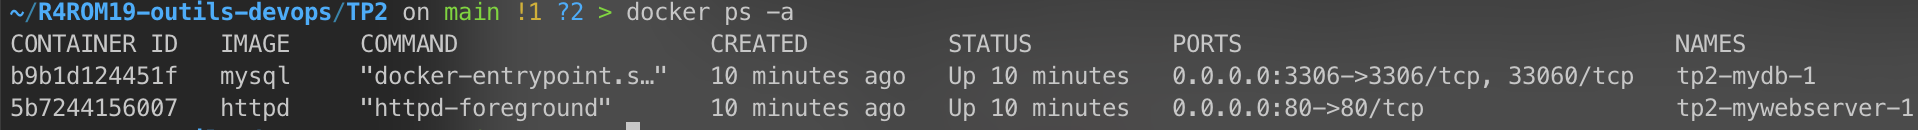
\includegraphics[width=1\textwidth]{img/ps-a.png}
    \caption{docker ps -all}
    \label{fig:ps-a}
\end{figure}\\

Je peux aussi bien entendu visualiser les logs avec \textbf{docker-compose logs}
\begin{figure}[h]
    \centering
    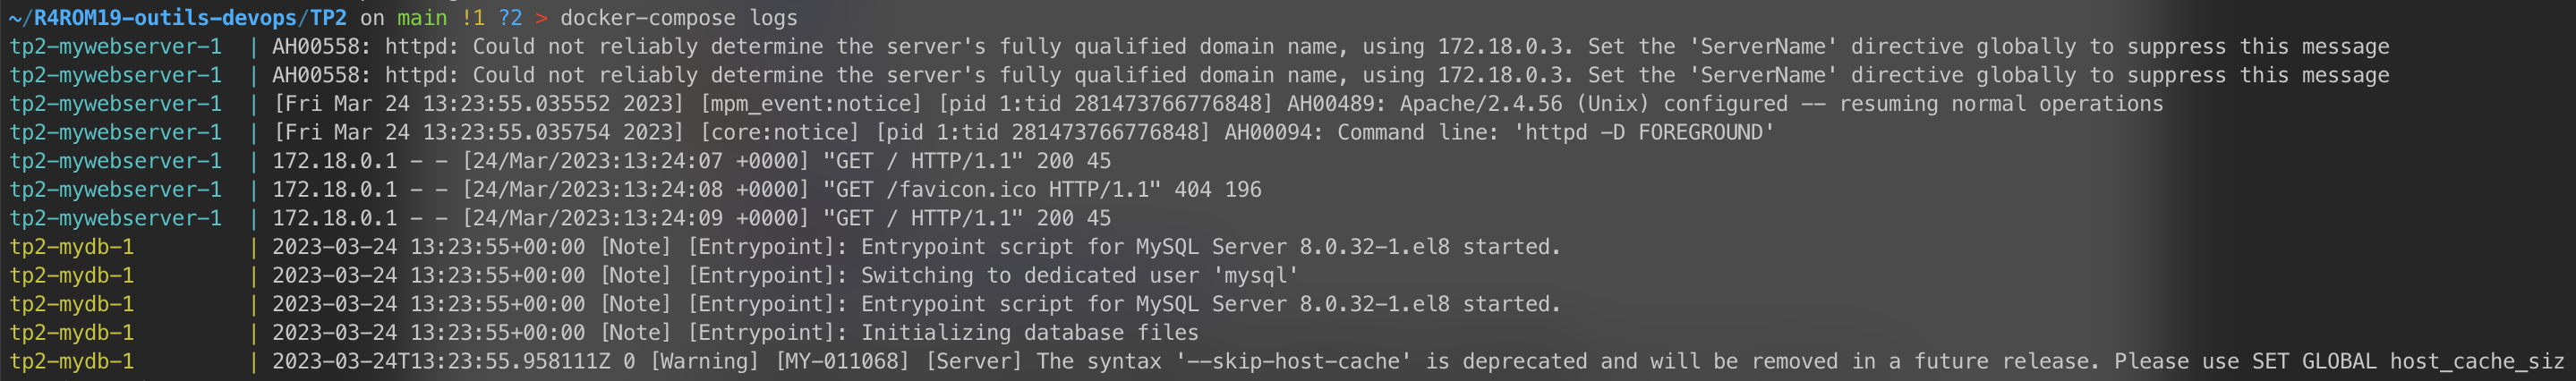
\includegraphics[width=1\textwidth]{img/logs.png}
    \caption{docker-compose logs}
    \label{fig:logs}
\end{figure}\\

\subsubsection{Question 5}
Je me connecte au docker avec la commande \textbf{docker exec -it tp2-mydb-1 /bin/bash}
On peut constater que j'atteris bien dans le docker en bash.
\begin{figure}[h]
    \centering
    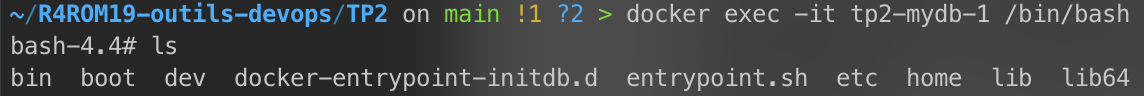
\includegraphics[width=1\textwidth]{img/connexion.png}
    \caption{Connexion à la base de données}
    \label{fig:connexion}
\end{figure}

\newpage
J'ai aussi bien évidemment accès la base de données en m'y connectant avec la commande \textbf{mysql -u root -p}
\begin{figure}[h]
    \centering
    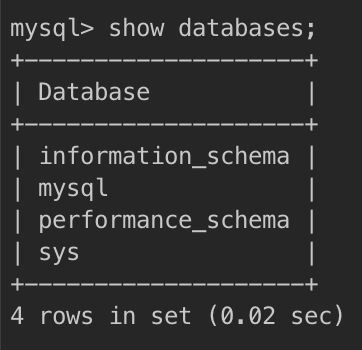
\includegraphics[width=0.4\textwidth]{img/bdd.png}
    \caption{Connexion à la base de données}
    \label{fig:bdd}
\end{figure}

\subsection*{Configuration de services interconnectés}
\subsubsection{Question 1-2}
Je viens donc modifier mon fichier de configuration du docker \textbf{docker-compose.yaml}.
de cette manière. 


\end{document}